\documentclass[]{article}
\usepackage[utf8]{inputenc}
\usepackage[margin=2cm]{geometry}
\usepackage{float}
\usepackage{framed}
\usepackage{fancyhdr}
\usepackage{amssymb}
\usepackage{xcolor}
\usepackage{amsmath}
\usepackage{cancel}
\usepackage[bottom]{footmisc}
\usepackage{titling}

% Define custom colours
\definecolor{cern-blue}{RGB}{0,51,160}
\definecolor{cern-violet}{RGB}{110,36,102}

\usepackage[colorlinks=true,citecolor=cern-blue,linkcolor=cern-violet,urlcolor=cern-blue]{hyperref}%
\usepackage{graphicx}
\usepackage{url}
\usepackage{tikz}
\usepackage{mathtools}
\usepackage{physics}
\usepackage[font=small, labelfont=bf]{caption}
\setlength{\droptitle}{-1.5cm}
\numberwithin{equation}{section}

% include bibliography in table of contents
\usepackage[backend=biber,style=ieee,sorting=none]{biblatex} % Using IEEE standard
\addbibresource{biblio.bib} % Point to the references folder
\renewcommand{\refname}{Bibliography}

\newcommand{\qedwhite}{\hfill \ensuremath{\Box}}
\renewcommand{\footrulewidth}{0.4pt}

\usepackage[most]{tcolorbox}
\definecolor{cern}{RGB}{155,174,219}

\tcbsetforeverylayer{
  fonttitle=\bfseries,
  left=.005\textwidth,
  right=.005\textwidth,
  breakable,
  enhanced,
  coltitle=white,
  colframe=cern,
  colback=white,
}

% Include coloured framing of examples
\usepackage{amsthm}
\newtheoremstyle{break}
  {\topsep}{\topsep}%
  {}{}%
  {\bfseries}{}%
  {\newline}{}%
\theoremstyle{break}
\newtheorem*{example}{Example}
\newtheorem*{definition}{Definition}
\newtheorem*{spproof}{Proof}
\usepackage[framemethod=TikZ]{mdframed}

\surroundwithmdframed[
  topline=false,
  rightline=false,
  bottomline=false,
  linecolor=cern-blue, 
  skipabove=\medskipamount,
  skipbelow=\medskipamount
]{example}

\surroundwithmdframed[
  topline=false,
  rightline=false,
  bottomline=false,
  linecolor=cern-violet, 
  skipabove=\medskipamount,
  skipbelow=\medskipamount
]{spproof}

\surroundwithmdframed[
  topline=false,
  rightline=false,
  bottomline=false,
  linecolor=black, 
  skipabove=\medskipamount,
  skipbelow=\medskipamount
]{definition}



\newcommand{\bk}{\par\null\par\noindent}


\title{\textbf{Investigation of the n-Vector Model}}
\author{Jakub Aleksander Kwaśniak}
\date{\today}

\fancypagestyle{plain}{
\fancyhead[R]{PPM 2024/2025}
\fancyhead[C]{n-Vector Model}
\fancyhead[L]{Numerical Methods for Physics}
}
\pagestyle{plain}

\begin{document}
\maketitle
\section{Introduction}
The n-vector model, also referred to as $O(n)$  model describes the interaction of classical spins on a lattice, developed as a generalisation of the Lenz-Ising model by H. E. Stanley in 1968 \cite{stanley-1968}. The relevant particular cases of the $n$-vector model are highlighted in the table \ref{tab:table} below.

\begin{table}[H]
    \centering
    \begin{tabular}{|c|c|}
         \hline  \boldmath $n$ \unboldmath &  \textbf{Name}\\ \hline 
         0 & Self-avoiding walk \\ \hline 
         1 &  Lenz-Ising model \\ \hline 
         2 &  XY Model \\ \hline 
         3 &  Heisenberg model \\ \hline 
         4 & Higgs sector model \\ \hline
    \end{tabular}
    \caption{Summary of particular cases of the $n$-vector model.}
    \label{tab:table}
\end{table}
The aim of this work is to provide insight behind the various $n$-cases, in direct comparison to the well-established Lenz-Ising model.

\section{Lenz-Ising Model ($n=1$)}
The Ising model, was first posed as a problem by Wilhelm Lenz in 1920 \cite{lenz-1920} to his student Ernst Ising, who then solved it as a part of his thesis in 1924 \cite{ising-1925}. 
\bk
The model consists of a $d$-dimensional lattice $\Lambda$ with a total of $N$ sites. Each site is assigned a value $\sigma_i = \pm 1$, resemblant of the orientation of the spin of a given magnetic material. At any given time, we describe the state of all lattice sites with a given configuration, or microstate, $\ket{\sigma_1 \sigma_2 \dots \sigma_N}$. The Hamiltonian functional describing the total energy of the configuration is given by \cite{cipra-1987}
\begin{equation}
 H(\sigma) = -\sum_{\langle i,j\rangle} J_{ij}\sigma_i \sigma_j - \mu \sum_i h_{i}\sigma_i, 
\label{eq:gen_H}
\end{equation}
where the summation convention $\langle i,j\rangle$ refers to summing over each pair of sites. This hints at a significant idealisation of the problem, where it is assumed that the interaction proceeds only through nearest neighbours on the lattice. Note also, that $\mu$ refers to the magnetic moment, $h_i$ the external magnetic field, and $J_{ij}$ the interaction strength. Depending on the sign of the latter, the material may be though of as a ferromagnet $(J_{ij} > 0)$ or an antiferromagnet ($J_{ij} < 0$).
\bk
Yet another simplification arises when the so-called zero-field case is considered, with no external magnetic field applied ($h_i = 0$ for all $i$). Furthermore, $J_{ij}$ may be assumed to be a constant $J$ for each pair of spins. The effective Hamiltonian is then
\begin{equation}
 H(\sigma) = -J \sum_{\langle i, j \rangle} \sigma_i\sigma_j.
\label{eq:red_H}
\end{equation}
By surrounding the system with a heat bath at a constant temperature $T$, it may be modelled in the canonical ensemble, with a probability of a given microstate given by the Boltzmann weight $p(\sigma) = e^{-\beta H(\sigma)}/Z$, where $Z$ is the canonical partition function,
\begin{equation}
Z = \sum_{\sigma} e^{-\beta H(\sigma)}.
\label{eq:partition}
\end{equation}
Using this formulation, macroscopic properties of the system may be computed,
\begin{equation}
E \equiv \langle H \rangle = \sum_{\sigma}H(\sigma) p(\sigma) = \frac{1}{Z}\sum_{\sigma}H(\sigma)e^{-\beta H(\sigma)} = -\frac{1}{Z}\frac{\partial Z}{\partial \beta} = -\frac{\partial \ln Z}{\partial \beta},
\label{eq:avg_E}
\end{equation}
\begin{equation}
M = \sum_{i=1}^{N} \sigma_i.
\label{eq:magnetisation}
\end{equation}

\begin{example}[One-dimensional Ising Model]
Consider for simplicity the situation with $d=1$ and $N = 3$, such that the Hamiltonian for the system is given by \cite{cipra-1987}
\[H(\sigma_1, \sigma_2, \sigma_3) = -J(\sigma_i\sigma_2 + \sigma_2\sigma_3).\]
Note that we have not introduced periodic boundary conditions, since in the thermodynamic limit it will not influence the result. Computing the partition function is equivalent to summing over the different values of $\sigma$.
\[Z = \sum_{\sigma_1=\pm1}\sum_{\sigma_2 = \pm1}\sum_{\sigma_3=\pm1}e^{-\beta H(\sigma_1, \sigma_2, \sigma_3)} = 2e^{2\beta J} + 2e^{-2\beta J} + 4 = 2^3\cosh^2(\beta J) = 2^N\cosh^{N-1}(\beta J)\]
This result, in fact is valid for any $N$ in the one-dimensional case. Moreover in the thermodynamic limit of $N$ large,
\begin{equation}
Z \approx (2\cos\beta J)^N.
\label{eq:1d_Z}
\end{equation}
\end{example}
\newpage

\section{Markov Chain Monte Carlo (MCMC) method}
In many areas of research, it is ubiquitous that the increasing complexity of physical problems implies lack of analytical solutions. Therefore, in order to analyse the behaviour of a given system, very often it is necessary to employ numerical methods. Among one of the most widely applicable schemes is the so-called Monte Carlo method, developed by the Polish mathematician Stanisław Ulam. Throughout this section, we follow the treatment of Kastner \cite{kastner-2010} to develop the theoretical treatment behind the employed algorithms.
\bk
Before defining the actual method, it is useful to review some concepts from probability theory.

\begin{definition}[Distribution]
A vector $\lambda = (\lambda_i: i\in S)$ is called a distribution on a state space $S$ if its elements $\lambda_i$ satisfy
\begin{enumerate}
    \item $\lambda_i \geq 0$ $\forall$ $i\in S.$
    \item $\sum_{i\in S} \lambda_i = 1.$
\end{enumerate}
\end{definition}
\begin{definition}[Stochastic matrix]
A matrix $T = (T_{ij}: i,j \in S)$ is called a stochastic matrix on $s$ if all its row vectors are distributions, such that
\begin{enumerate}
    \item $T_{ij} \geq 0$ $\forall$ $i,j \in S$.
    \item $\sum_{i\in S} T_{ij} = 1$ $\forall$ $j\in S$.
\end{enumerate}
\end{definition}
\begin{definition}[Stationary distribution]
A stationary distribution of a stochastic matrix $T$ is a distribution $\pi = (\pi_i : i \in S)$, such that
\[T \pi = \pi,\]
i.e., $\pi$ is an eigenvector of the matrix with eigenvalue unity.
\end{definition}
\begin{definition}[Detailed balance]
Let $A = (A_{ij}: i,j\in S)$ be a matrix and $\pi = (\pi_{i} : i\in S)$ be a vector. $A$ is said to satisfy detailed balance with respect to $\pi$ if
\[A_{ij}\pi_j = A_{ji}\pi_i\]
for all $i,j \in S$.
\end{definition}
\bk
Having introduced the preliminary notions, we may begin developing the Monte Carlo method itself. For example, in equilibrium statistical physics, many quantities are calculated using a sum or an integral over a certain space. The main idea is to replace this large summation over the entire space by a summation over a randomly chosen subspace of it. In introducing the stochastic nature of the method, one may define the so-called Markov Chain
\begin{definition}[Markov Chain]
Let $T$ be a stochastic matrix and $X_n$ a random variable defined in a space $S$. The sequence of random variables $\{X_n\}\equiv\{X_0, X_1, \dots, X_{N-1}\}$, is called a Markov Chain of length $N$ on $S$ with a transition matrix $T$ and initial distribution $\lambda$ if
\begin{enumerate}
    \item $X_0$ has distribution $\lambda$.
    \item For $n\geq 1$, given $X_n$ having distribution $j$, $X_{n+1}$ has distribution $T_{ij}, $ for any $j\in S$.
\end{enumerate}
\end{definition}
The full sequence of random variables may be represented as follows using a Markovian approach
\[\{X_n\} = \{\lambda, T\lambda, T^2\lambda, \dots, T^{N-1}\lambda\}.\]
This implies that the distribution of $X_{n+1}$ depends only on $X_n$. Commonly, it is said that the Markov Chain "has no memory", which provides an argument for its efficiency in computations. Effectively, the aforementioned summation over the entire state space of the system may be replaced by a sum over the Markov Chain on that same state space. This will provide an estimation of the actual value in question, dependent on the characteristics of the chain. 

\begin{definition}[Monte Carlo estimator]
    Let $F = \sum_{i\in S}f(i)$ be some function to be computed. We call
    \[\tilde{F} = \frac{1}{N}\sum_{i\in \{X_n\}}\frac{f(i)}{\pi_i}\]
    the Monte Carlo estimator of $F$, where $\{X_n\}$ the Markov Chain of length $N$ on $S$, and $\pi = (\pi_i : i\in S)$ with $\pi_i > 0$, is the stationary distribution of the transition matrix $T$.
    \end{definition}
    
    \bk
    \noindent To illustrate the application of the Monte Carlo method, consider the standard example from classical statistical physics.
    \bk 
    
    \begin{example}[Canonical ensemble]
    Recall the expectation value of the energy in the canonical ensemble
    \[\langle H \rangle = \frac{1}{Z(\beta)}\sum_{i\in S}H(i)e^{-\beta H(i)},\]
    where $Z(\beta)$ is the partition function
    \[Z(\beta) = \sum_{i\in S}e^{-\beta H(i)}.\]
    If we define
    \[f(i) \equiv \frac{1}{Z(\beta)} H(i)e^{-\beta H(i)}, \]
    and
    \[\pi = (\pi_i = e^{-\beta H(i)}/Z(\beta): i\in S),\]
    then the expression for the expectation value may be obtained from the Monte Carlo estimator,
    \[\tilde{E} = \frac{1}{N}\sum_{i\in\{X_n\}}H(i).\]
    As we can see, this value is dependent on the length of the Markov Chain $n$, as well as the actual random variables itself, which are determined by the initial distribution $\lambda$ and the transition matrix $T$.
    \end{example}
\bk
    In most applications, the problem in developing the Monte Carlo algorithm reduces to finding an appropriate transition matrix. One such method is the so-called Metropolis-Hastings algorithm, pioneered by Nicholas Metropolis et al. (including Edward Teller) in 1953 \cite{metropolis-1953} and Wilfred Hastings in 1970 \cite{hastings-1970}. 
    \bk The method relies on constricting the transition probabilities from a proposal matrix $P$ and an acceptance matrix $A$. Suppose we start with a random variable $X_n = j$ as an element of a Markov Chain. The probability of the next element of the chain being $i$ is proposed to be $P_{ij}$, an element of the proposal matrix. If the proposal is accepted, set $X_{n+1} = i$ with probability $A_{ij}$. If it is rejected, set $X_{n+1} = j$ with probability $1-A_{ij}.$ The elements of the transition matrix may be written as
    \begin{equation}
    T_{ij} = P_{ij}A_{ij} + \delta_{ij} \sum_{k\in S}P_{kj}(1-A_{kj}).
    \label{eq:T_mat}
    \end{equation}
In order for $T$ to be a properly defined stochastic matrix with stationary distribution $\pi$, it needs to fulfil certain conditions for all $i, j \in S$:
\begin{enumerate}
    \item $P$ is symmetric ($P_{ij} = P_{ji}$).
    \item $P$ is stochastic.
    \item $0 \leq A_{ij} \leq 1$.
    \item $A$ satisfies the detailed balance condition.
\end{enumerate}
Furthermore, one may define the so-called acceptance function $f(z): (0, \infty) \rightarrow [0,1] $ such that $f(z) = z f(1/z)$. This way, the elements $A_{ij} = f(\pi_i/\pi_j)$ satisfy detailed balance.
\bk 
\subsection{Metropolis-Hastings acceptance function}
One common choice of the acceptance function is
\begin{equation}
f(z): z\mapsto \min(1,z).
\label{eq:mh_function}
\end{equation}
Using this specific form of the function, we may consider an example of the algorithm for two spins on a one-dimensional lattice.
\begin{example}[One-dimensional Ising Model: Metropolis-Hastings]
    The state space of the system $S$ is spanned by two degrees of freedom, corresponding to the two spins, $\sigma_1$ and $\sigma_2$, which take values $1$ or $-1$. It may be written as a direct product
    \[S = \{-1, 1\} \times \{-1, 1\}.\]
    For notational simplicity, we will denote the basis vectors of $S$ as
    \[1 \equiv 1 \times 1,\]
    \[2 \equiv 1 \times -1,\]
    \[3 \equiv -1 \times 1,\]
    \[4 \equiv -1 \times -1.\]
    The Hamiltonian of the Ising model may be written in terms of the spins, up to a constant of proportionality
    \[H(\sigma_1, \sigma_2) = \sigma_1\sigma_2.\]
    From this, we are able to construct the transition matrix for the Markov Chain applied in the Monte Carlo algorithm for the problem. Employing the notation where $T_{ij}$ represents the probability of transition from state $1$ to state $2$, we make the following choice for the proposal matrix
    \[P = \frac{1}{2}\begin{pmatrix}
        0 & 1 & 1 & 0 \\
        1 & 0 & 0 & 1 \\
        1 & 0 & 0 & 1 \\
        0 & 1 & 1 & 0 
    \end{pmatrix}.\] 
    As we saw in the canonical ensemble example, the stationary distribution may be chosen to be proportional to the Boltzmann weight
    \[\pi_i \propto e^{-\beta H(i)} \in \{e^{\beta}, e^{-\beta}\}.\]
    Utilising the acceptance function $f(z) = \min(1, z)$, the acceptance matrix $A$ may be calculated by noting $A_{ij} = \min(1, \pi_j/\pi_i)$,
    \[A = \begin{pmatrix}
        1 & 1 & 1 & 1\\
        e^{-2\beta} & 1 & 1 & e^{-2\beta} \\
        e^{-2\beta} & 1 & 1 & e^{-2\beta} \\
         1 & 1 & 1 & 1
    \end{pmatrix}.\]
    Directly from these expressions, using equation \eqref{eq:T_mat} allows for constructing the transition matrix
    \[T = \frac{1}{2}\begin{pmatrix}
        2(1-e^{-2\beta}) & 1 & 1 & 0 \\
        e^{-2\beta} & 0 & 0 & e^{-2\beta} \\
        e^{-2\beta} & 0 & 0 & e^{-2\beta} \\
        0 & 1 & 1 & 2(1-e^{-2\beta})
    \end{pmatrix}.\]
    In real applications it suffices to put forward a proposal for the next state and calculate the acceptance rate for the next state in the Markov chain. Notice that $A$ may be written more compactly by defining $\Delta H = H_j - H_i$
    \[A = \begin{cases}
        e^{-\beta\Delta H} \quad \text{ if } \Delta H > 0 \\
        1\quad\quad\quad\quad\quad \text{ else}
    \end{cases}.\]
    From this expression, we may note that the Metropolis-Hastings algorithm, given a current state of the spin proposes to map the spin onto its opposite value with a probability $1$ if the energy of the next state is lower than the previous one. Otherwise, if the energy is larger, there is still a probability of the spin flipping, being $e^{-\beta(H_j - H_i)},$ corresponding physically to random thermal fluctuations in the system. The plot of the function may be found in figure \ref{fig:metropolis} below.
    \begin{figure}[H]
        \centering
        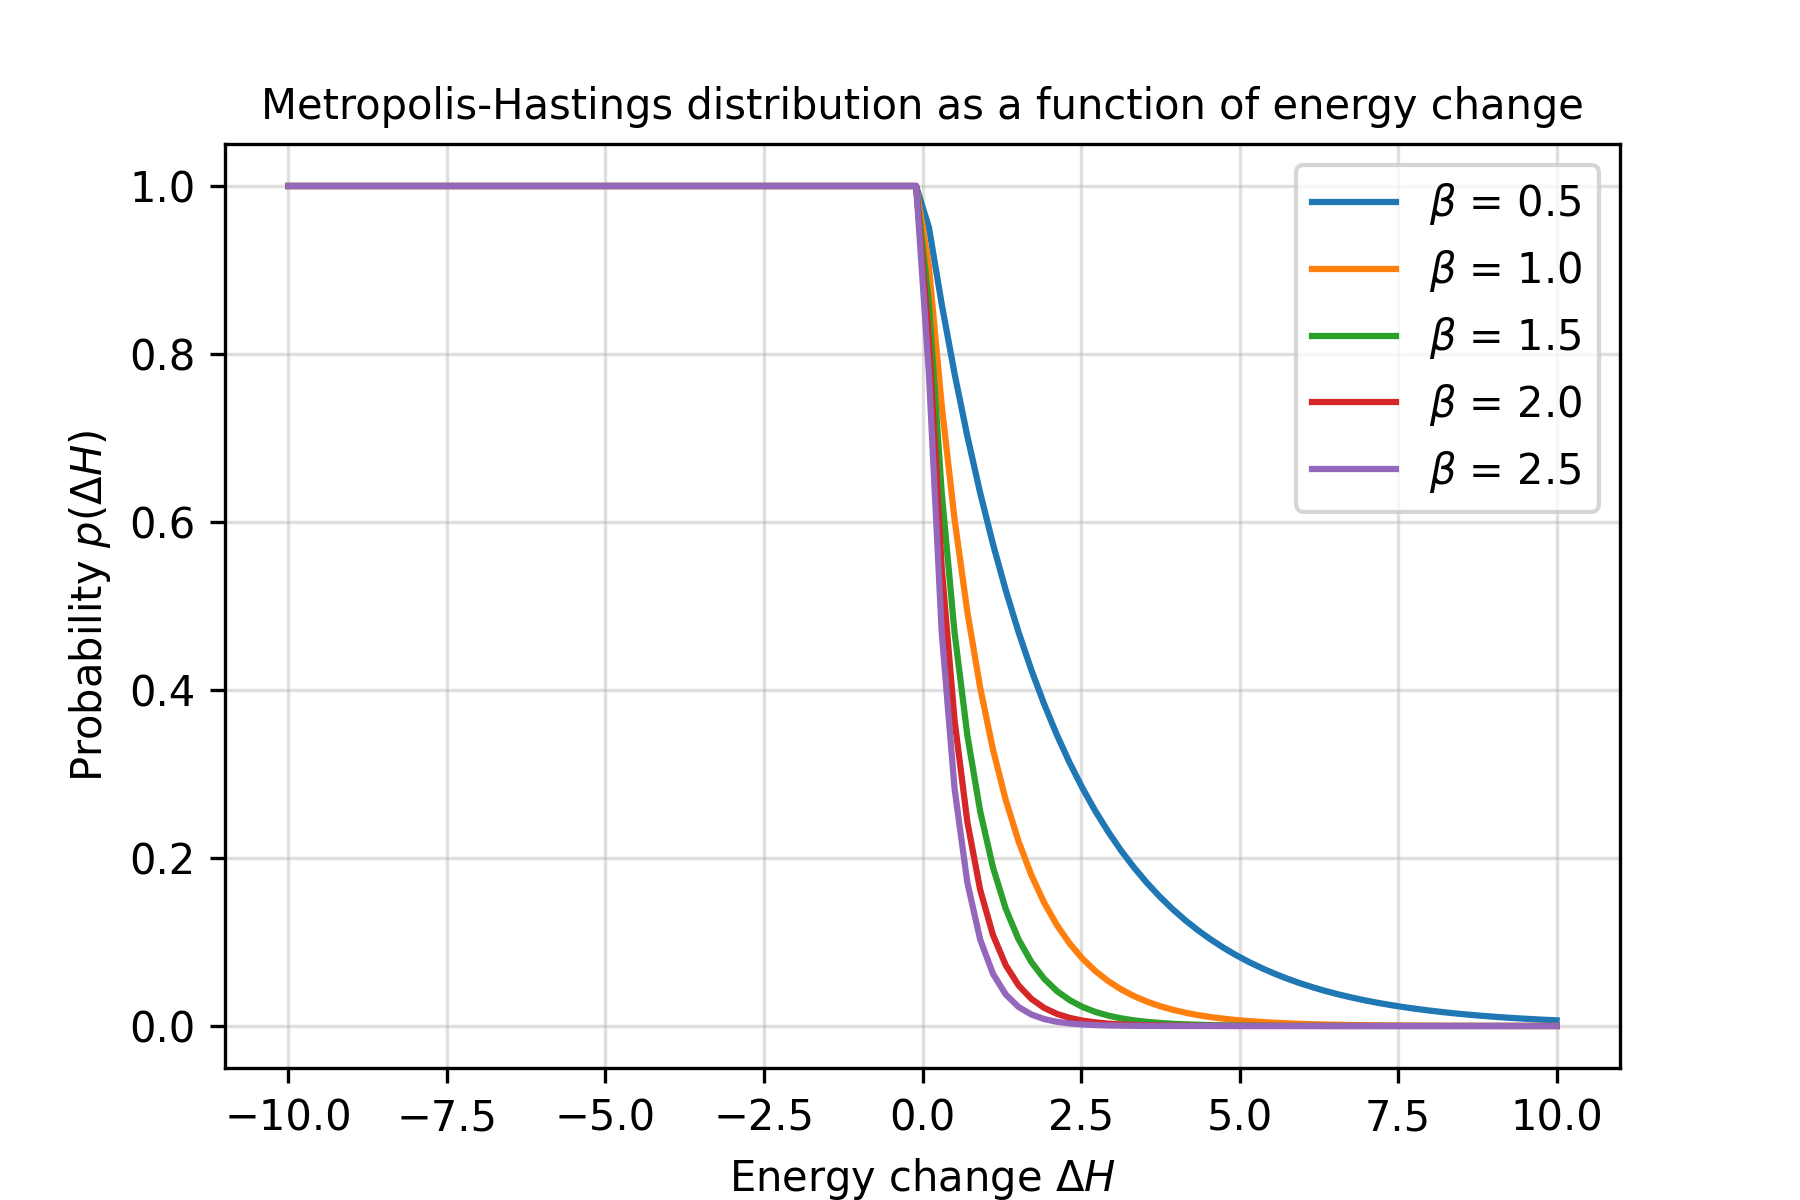
\includegraphics[scale=0.7]{figures/metropolis.png}
        \caption{Plot of the Metropolis-Hastings distribution as a function of energy change, for various values of the inverse temperature $\beta$.}
        \label{fig:metropolis}
    \end{figure}
\end{example}
\subsection{Glauber acceptance function}
An alternative to the Metropolis-Hastings function is the so-called Glauber function
\begin{equation}
f(z): z \mapsto \frac{z}{1+z}.
\label{eq:glauber}
\end{equation}
To directly compare the approach with the previous algorithm, consider the same example of two spins on a one-dimensional lattice.
\begin{example}[One-dimensional Ising Model: Glauber]
The set-up of the problem is exactly the same as before, with the same proposal matrix $P$ and the stationary distributions $\pi_i$. The acceptance matrix now may be calculated using equation \eqref{eq:glauber}
\[A_{ij} = \frac{\frac{\pi_j}{\pi_i}}{1 + \frac{\pi_j}{\pi_i}} = \frac{\pi_j}{\pi_i + \pi_j}.\]
In complete matrix form, $A$ may be represented as follows
\[A = \frac{1}{2}\begin{pmatrix}
    1 & \frac{2}{1+e^{-2\beta}} & \frac{2}{1+e^{-2\beta}} & 1 \\
    \frac{2}{1+e^{2\beta}} & 1 & 1 & \frac{2}{1+e^{2\beta}} \\
    \frac{2}{1+e^{2\beta}} & 1 & 1 & \frac{2}{1+e^{2\beta}} \\
    1 & \frac{2}{1+e^{-2\beta}} & \frac{2}{1+e^{-2\beta}} & 1
\end{pmatrix}.\]
A given spin state will flip, according to the proposal condition, with a different probability than the one of Metropolis. Notably, it is not sure that the spin will flip, even if the configuration yields a more energetically favourable arrangement. $A$ may be written more compactly
\[A = \begin{cases}
    (1+e^{\beta\Delta H})^{-1} \quad \text{ if } \Delta H \neq 0 \\
   \quad \quad 1/2\quad\quad\quad\quad\quad \text{ else}
\end{cases}.\]
Therefore, the probability of the spin flip occurring is simply the Glauber function \eqref{eq:glauber} with $z = e^{\beta H}$
\[p(\Delta H) = \frac{1}{1+e^{\beta \Delta H}}.\]
The plot of the function is provided in figure \ref{fig:glauber} below.
\begin{figure}[H]
    \centering
    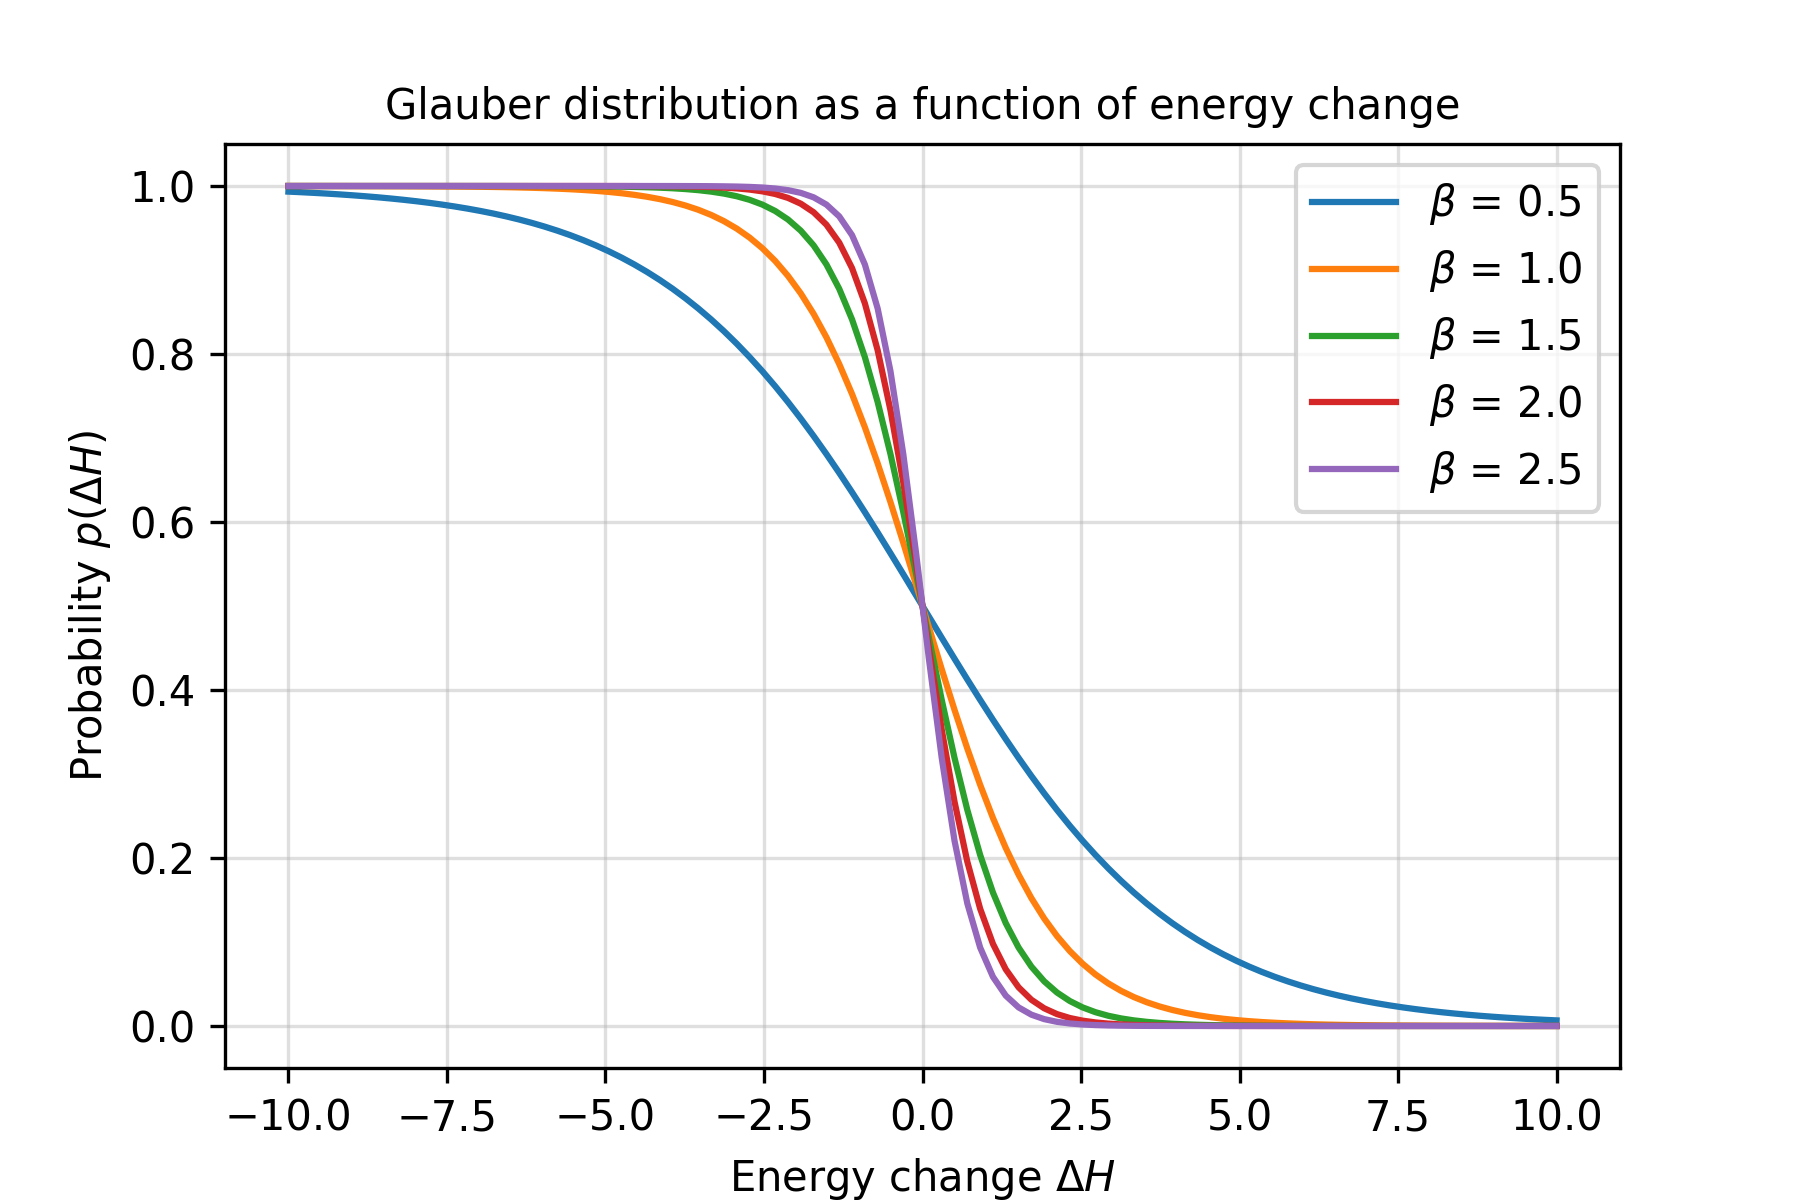
\includegraphics[scale=0.7]{figures/glauber.png}
    \caption{Plot of the Glauber distribution as a function of energy change, for various values of the inverse temperature $\beta$.}
    \label{fig:glauber}
\end{figure}

\noindent Comparing this plot with figure \ref{fig:metropolis}, we may notice that both probability distributions converge to a step function at low temperatures (large $\beta$), and hence are perfectly equivalent in this regime. Moreover, they should yield the same results at thermal equilibrium. The differences between the two algorithms become important at high temperatures. Nevertheless, they both satisfy ergodicity and the detailed balance conditions. 
\end{example}
\newpage
\section*{Bibliography}
\printbibliography[heading=none]

\end{document}